%!TeX root = ./../MusterAbschlussarbeit.tex

%##########################################################
% Inhalt
%##########################################################

\clearpage
\chapter{Implementation}

\section{Umsetzung in Unity}
Der \textbf{Controller} stellt alle Funktionalitäten bereit, welche gebraucht werden um die Lernumgebung zu initialisieren.
Er besitzt Prefabs des Agents, des GameFields und der Würfel und initialisiert diese zum Start.
Weiterhin implementiert der Controller die Funktionalität der Punktevergabe, welche für eine Mehrspielervariante genutzt werden kann.
Der Controller ist das Parent aller anderen Elemente und so ist er das Zentrale Element der Steuerung. Auch das wiederholte rollen der Würfel wird im Controller angestoßen.
Der Controller war sehr hilfreich beim erstellen paralleler Trainings, da dieser einfach mehrfach in die Szene aufgenommen werden musste um mehrere Spielfelder, welche gleichzeitig bespielt werden zu initialisieren.

<Code ausschnitt?>

Der \textbf{NumberDice} implementiert die Logic, welche für das Würfeln und Visualisieren der Zahlenwürfel benötigt wird.
Die Visualisierung funktioniert mit selbst angefertigten Sprites welche in einem Sortierten Array liegen und je nach gewürfelter Zahl initialisiert und gerendert werden.
Beim wiederholten Würfeln, wird das initialisierte Sprite destroyed und ein neues erzeugt.
Damit ist gewährleistet, dass immer das aktuelle Würfelergebnis angezeigt wird.
Die Zahl des Würfels wird als Integer wert gespeichert, wobei er die Zahlen 1-6 annehmen kann.
Die Zahl sechs entspricht dem Zahlenjoker.

<Code>

Wie der Zahlenwürfel implementiert der \textbf{ColorDice} die Funktionalität des Würfelns der Farben.
Diese werden als String dargestellt und kann folgende Werte annehmen: \{'blue', 'green','red', 'yellow', 'orange', 'joker'\}
Zur Visualisierung wird ein Sprite erstellt, was in der gewürfelten Farbe eingefärbt wird.
Ein schwarzes Feld entspricht dem gewürfelten Farbjoker.

<Code>

Das \textbf{GameField} stellt das tatsächliche Spielfeld dar.
Es implementiert die benötigten Methoden um die SquareFields zu verwalten und rückzusetzen.
Außerdem wird die Anzahl der Joker in ihm gehalten.

Funktionalitäten:
\setlist{noitemsep}
\begin{itemize}
	\item  Visualisierung des Spielfeldes
    \item  Aktualisieren der Gruppen aller Felder
    \item  Abkreuzen der Felder
    \item  Berechnen der validen Nachbarn der Felder
    \item  Berechnen der verbleibenden Felder einer bestimmten Farbe
    \item  Rückgabe der validen Felder für die aktuell gewählten Würfel.
    \item  Reduzieren der verbleibenden Joker
    \item  Rücksetzen der Felder um ein neuest Spiel zu Starten
\end{itemize}

Die \textbf{FieldSquares} stellen die einzelnen Teilfelder des Spielfeldes dar.
Gehaltene Informationen:
\begin{table}[htbp]
    \centering
    \begin{tabular}{|c|c|c|}
    \hline
    \textbf{Beschreibung} & \textbf{Typ} & \textbf{Wertebereich} \\
    \hline
    Feld ist ein Sternfeld & Boolean & True / False \\
    \hline
    Farbe des Feldes & String & - \\
    \hline
    Feld ist ausgefüllt & Boolean & True / False \\
    \hline
    Feld ist verfügbar & Boolean & True / False \\
    \hline
    Clustergröße & Integer & 1-6 \\
    \hline
    X-Koordinate des Feldes & Integer & 0-14 \\
    \hline
    Y-Koordinate des Feldes & Integer & 0-6 \\
    \hline
    \end{tabular}
    \caption{Beschreibung, Typ und Wertebereich der Feldinformationen}
    \label{tab:field_info}
\end{table}

\subsection{Visualisierung}
Die Visualisierung des Spielfeldes erfolgt über ein angefertigtes Prefab. In diesem wurden die 105 Kästchen in einem Raster von 15x7 instanziiert und manuell mit den Informationen versehen. Dieses manuell angefertigte Spielfeld wurde als Prefab gespeichert und dient als Umgebung für den Agenten.
Zu Beginn des Spiels, werden die Felder in die Farben der hinterlegten Information in den richtigen Farben eingefärbt. Ausgefüllte Kästchen werden grau eingefärbt, diese Funktionalität wird im Fieldsquare Prefab ausgeführt.

<Code instanziierung der Felder?>

<Code einfärben der Felder>

\section{Implementierung des Agenten}
Der Agent ist die Schnittstelle zwischen dem Environment und dem RL.
Dem Agent werden alle nötigen Informationen des Spielfeldes übergeben. Diese werden in ein Neuronales Netz übertragen, welches wiederum die Ausgabewerte in einem Vektor zurück an den Agent leitet.
Anschließend wird der Vektor verarbeitet und die gewählten Aktionen werden ausgeführt.
Für gute Aktionen erhält der Agent positive Rewards, bei schlechten Aktionen wird der Zug übersprungen. \\
Zu Beginn jeder Episode, welche einem Spielzug entspricht, muss dem Agenten der aktuelle Zustand des Feldes übermittelt werden, aus welchem er die bestmögliche Option für einen Zug berechnet. In der ML Agents Bibliothek gibt es hierfür eine vorgefertigte Methode mit dem Namen CollectObservations. Die bearbeitet einen Observationsvektor zu welchem die Informationen hinzugefügt werden.
Wärend des Trainings eines Neuronalen Netzes, muss die Anzahl der Observations gleich bleiben. Das bedeutet es ist nicht ohne weiteres möglich ein Model auf unterschiedlichen Spielfeldern zu trainieren, da sich so die Anzahl der Observations unterscheiden würden.


Aufbau der Observations:
\begin{table}[htbp]
    \centering
    \begin{tabular}{|c|c|c|c|}
    \hline
    \textbf{Index} & \textbf{Beschreibung} & \textbf{Type} & \textbf{Wertebereich} \\
    \hline
    0 & Anzahl der verbleibenden Joker & Float & $[0 - 1]$ \\
    \hline
    1 & Anzahl der gespielten Runden & Float & $[0 - 1]$ \\
    \hline
    2 & Ergebnis des ersten Zahlenwürfels & Float & $[0 - 1]$ \\
    \hline
    3 & Ergebnis des zweiten Zahlenwürfels & Float & $[0 - 1]$ \\
    \hline
    4-9 & Ergebnis des ersten Farbwürfels & Vector6 (Binary) & $(0, 1)^6$ \\
    \hline
    10-15 & Ergebnis des zweiten Farbwürfels & Vector6 (Binary) & $(0, 1)^6$ \\
    \hline
    16-24 & Informationen für Feld 1 & - & - \\
    \hline
    25-33 & Informationen für Feld 2 & - & - \\
    \hline
    ... & ... & ... & ... \\
    \hline
    953-961 & Informationen für Feld 105 & - & - \\
    \hline
    \end{tabular}
    \caption{Zusammenfassung der Observations und Feldinformationen}
    \label{tab:combined_table}
\end{table}
    
\begin{table}[htbp]
    \centering
    \begin{tabular}{|c|c|c|c|}
    \hline
    \textbf{Stelle im Vektor} & \textbf{Beschreibung} & \textbf{Type} & \textbf{Wertebereich} \\
    \hline
    $k+16$ - $k+21$ & Farbe des Feldes $k$ & Vector6 (Binary) & $(0, 1)^6$ \\
    \hline
    $k+22$ & Ist Feld $k$ verfügbar & Boolean & True / False \\
    \hline
    $k+23$ & Ist Feld $k$ abgestrichen & Boolean & True / False \\
    \hline
    $k+24$ & Ist Feld $k$ ein Sternfeld & Boolean & True / False \\
    \hline
    \end{tabular}
    \caption{Observation jedes einzelnen Feldes}
    \label{tab:field_variables}
\end{table}

<skript Collect Observations> \\
Anhand der Observations berechnet das Neuronale Netz einen Ausgabevektor. Mit diesem führt der Agent nun bestimmte Aktionen aus und versucht sein Ergebnis (Rewards) zu maximieren.
Anhand der gesammelten Rewards wird das Neuronale Netz nun angepasst um das bestmögliche Ergebnis zu erreichen.


Aufbau Actionbuffer:
\begin{table}[htbp]
    \centering
    \caption{Index und Beschreibung der Variablen}
    \begin{tabular}{|c|c|c|c|}
    \hline
    \textbf{Index} & \textbf{Beschreibung} & \textbf{Typ} & \textbf{Wertebereich} \\
    \hline
    \textbf{1} & Index des gewählten ZahlenWürfels & Integer & 0-1 \\
    \hline
    \textbf{2} & Index des gewählten Farbwürfels & Integer & 0-1 \\
    \hline
    \textbf{3} & Jokerzahl & Integer & 0-4 \\
    \hline
    \textbf{4} & X-Koordinate des gewählten Feldes & Integer & 0-14 \\
    \hline
    \textbf{5} & Y-Koordinate des gewählten Feldes & Integer & 0-7 \\
    \hline
    \textbf{6} &  Action 1 für die Auswahl der Nachbarn & Continuous & - \\
    \hline
    \textbf{7} &  Action 2 für die Auswahl der Nachbarn & Continuous & - \\
    \hline
    \textbf{8} &  Action 3 für die Auswahl der Nachbarn & Continuous & - \\
    \hline
    \textbf{9} &  Action 4 für die Auswahl der Nachbarn & Continuous & - \\
    \hline
    \end{tabular}
    \label{tab:variables}
\end{table}

\newpage
\subsection{Erklärung des Alghorithmus}
Im folgenden wird der Ablauf zum Wählen der Felder erläutert. Im Beispiel wird der Ausgabevektor \textbf{(1 , 1 , 0 , 3 , 4 , 0.6 , 0.5 , 0.4 , 0.8)} verwendet. \\
Die ersten beiden Stellen des Ausgabevektors entsprechen den gewählten Würfeln.
Im ersten Schritt werden alle Feldes des Spielfedes untersucht, ob sie ein valides Ziel für das gewürfelte Ergebnis bilden.
Die ergibt sich aus der Gruppe der Spielfelder, der Farbe und ob das Kästchen verfügbar ist.
Valide Felder werden in eine Liste (availableFields) aus Verfügbaren Feldern geschrieben.

\begin{figure}[!h]
	\centering
	\includegraphics[width=0.5\textwidth]{Bilder/Erklärung_Alghorhitmus_1.png}
	\caption{Valide Felder für das gewählte Würfelergebnis wurden markiert}
\end{figure}

Anschließend wird geprüft, ob die gewählten Koordinaten in availableFields vorhanden sind.
Wenn nein wird die Episode abgebrochen und der Agent überspringt seinen Zug.
Sofern der Agent ein valides Feld gewählt hat, wird dieses in eine weitere Liste (pickedFields) geschrieben und benachbarte Felder der selben Gruppe werden zurückgegeben.

\newpage
\begin{figure}[!h]
	\centering
	\includegraphics[width=0.5\textwidth]{Bilder/Erklärung_Alghorhitmus_2.png}
	\caption{Feld(3,4) wird in die pickedField Liste aufgenommen und benachbarte Felder werden zurückgegeben.}
\end{figure}

Im nächsten Schritt wird jedem der verfügbaren Nachbarn abhängig der Gesamtanzahl ein Wertebereich zwischen 0 und 1 zugewiesen. Anhand des discreten Wertes des Ausgabevektors wird das Zugehörige Feld in pickedFields geschrieben.
\begin{table}[htbp]
    \centering
    \begin{tabular}{|c|c|c|}
    \hline
    \textbf{FeldKoordinaten} & \textbf{von} & \textbf{bis} \\
    \hline
    (3,5) & 0 & 0.33 \\
    \hline
    (4,4) & 0.33 & 0.66 \\
    \hline
    (3,3) & 0.66 & 0.99 \\
    \hline
    \end{tabular}
    \caption{Bereiche für bestimmte Felder}
    \label{tab:field_ranges}
\end{table}

\begin{figure}[!h]
	\centering
	\includegraphics[width=0.5\textwidth]{Bilder/Erklärung_Alghorhitmus_3.png}
	\caption{Feld(4,4) ist das nächste gewählte Feld und wird in pickedFields aufgenommen}
\end{figure}

Für alle Feldes in Picked Field werden die benachbarten Felder zurückgegeben und der vorherige Schritt wiederholt.
Wenn so viele Felder gewählt wurden, wie erwürfelt wurden, werden die Felder anschließend ausgefüllt und auf Rewards überprüft.

\begin{figure}[!h]
	\centering
	\includegraphics[width=0.5\textwidth]{Bilder/Erklärung_Alghorhitmus_4.png}
	\caption{Felder wurden gewählt und ausgefüllt}
\end{figure}


\newpage


\section{Trainingsversuche}
\subsection{Trainingsversuche}

Aufbau Actionbuffer bis dato -> würfel, würfel, feldIndex, feldIndex , feldIndex ,feldIndex, feldIndex (feldIndex int)
In den ersten Trainings soltle der Agent Würfel und anschließend zufällige Felder wählen.
Danach wurde überprüft ob alle ausgewählten Felder folgende Kriterien erfüllten:
\setlist{noitemsep}
\begin{itemize}
\item alle Felder verfügbar
\item alle Felder benachbart
\item alle Felder der selben farbe
\end{itemize}

Illegale Züge wurden bestraft (negative Rewards) und wurden nicht ausgeführt.
Da der Agent Anfangs zufällige Felder auswählt, hatte es zur Folge, dass nahezu keine Spielzüge getätigt wurden.
Dies führte dazu, dass das Spiel nicht gespielt wurde.
Dementsprechend war das Training auf diese Weise nicht erfolgreich und musste überarbeitet werden.


\subsection{Training des Agenten mit Zusatz Belohnungen}
In den Bereits erläuterten Trainingsversuchen, bekam der Agent für vermeintlich gute Züge eine Belohnung und für schlechte Züge eine Bestrafung.

- Für das Abkreuzen von Feldern 0.02f pro feld
- falls ein gesammmtes Cluster abgekreuzt wird -> 0.04 pro feld
- wahl eines Würfelpaars für das es keine legalen Züge gibt -> -50.0f
- Wahl eines Jokers obwohl keine Joker verfügbar sind -> -50.0f

Die Belohnungen führten dazu, dass der Agent nicht Versuchte Spalten abzukreuzen, da er das abkreuzen von Clustern für deutlich effizienter hielt um siene Belohnungen zu maximieren.
Obwohl die Belohnungen für Erreichte Spalten oder komplett ausgefüllte Farben mehr Punkte ergaben.


\begin{figure}[!t]
    \centering
    \includegraphics[scale=0.6]{Bilder/average_points.png}
    \caption{Das Logo von Informatik und Medien }
\end{figure}

\begin{figure}[!t]
    \centering
    \includegraphics[scale=0.6]{Bilder/average_rewards.png}
    \caption{Das Logo von Informatik und Medien }
\end{figure}

Die Grafiken zeigen deutlich, dass je länger der Agent tranierte desto kleiner die Durchschnittlichen Punkte pro Spiel wurden.
Dies spricht dafür, dass es zum sogenannten 'reward hacking' gekommen ist. Dieses Phänomen tritt auf, wenn der Agent sein eigentliches Ziel nicht erreichen kann, da er eine andere (falsche) Strategie erlernt, welche nicht zum eigentlichen Ziel führt. Ursache hierfür ist, dass der Agent sein eigentliches Ziel (das ausfüllen von Spalten) nie erreicht und somit nicht erlernt.


\section{Untersuchung des Trainingsfortschritts}
In diesem Versuch wird Untersucht ob das Training des Agenten erfolgreich war. In jeder Messreihe wurden 1Mio. Lernschritte druchgeführt was ca 33k gespielten Spielen entspricht. Im Anschluss wurde aus den gespielten Spielen die durchschnittliche erreichte Punktzahl kalkuliert und in einem Graphen dargestellt.

\subsection{Trainiert vs Untrainiert}
In diesem Experiment, werden die erreichten Punkte und Rewards eines untrainierten Agenten gegenüber den erziehlten Ergebnissen eines trainierten Agenten gegenübergestellt. Der trainierte Agent hat bereichts 25 Mio. Spielzüge absolviert, was ungefähr 830k gespielten Spielen entspricht.
Der untrainierte Agent bekommt ein neu initialisiertes NN, welches zufällig gewählte Kantengewichte zwischen den Neuronen erhält.
Wie an den Graphen zu erkennen ist, hat der trainierte Agent tatsächlich einen höheren Durchschnitt an erzielten Punkten pro Spiel. Auch die gesammlten Rewards sind bei dem trainierten Agenten höher.
Dies liegt daran, dass die Rewards so festgelegt sind, dass der Agent sie nur erhält, wenn er auch im Spiel punktet.
Schon während des Trainings war ein merklicher Unterschied festzustellen, deshalb war das Ergebnis dieses Experiments zu erwarten.


\begin{figure}[!t]
    \centering
    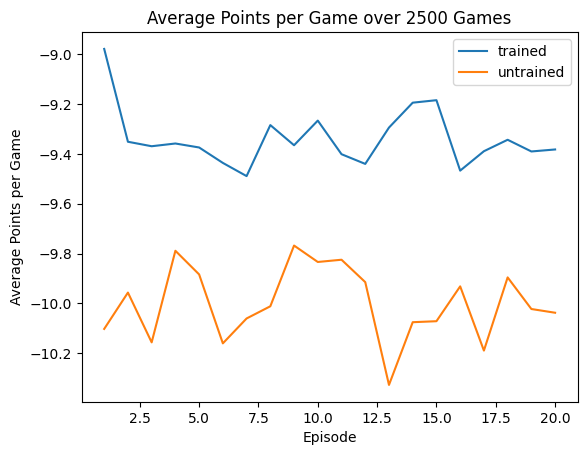
\includegraphics[scale=0.6]{Bilder/Points_trained_vs_untrained.png}
    \caption{Durchschnitt der erreichten Punkte pro Spiel }
\end{figure}
\begin{figure}[!th]
    \centering
    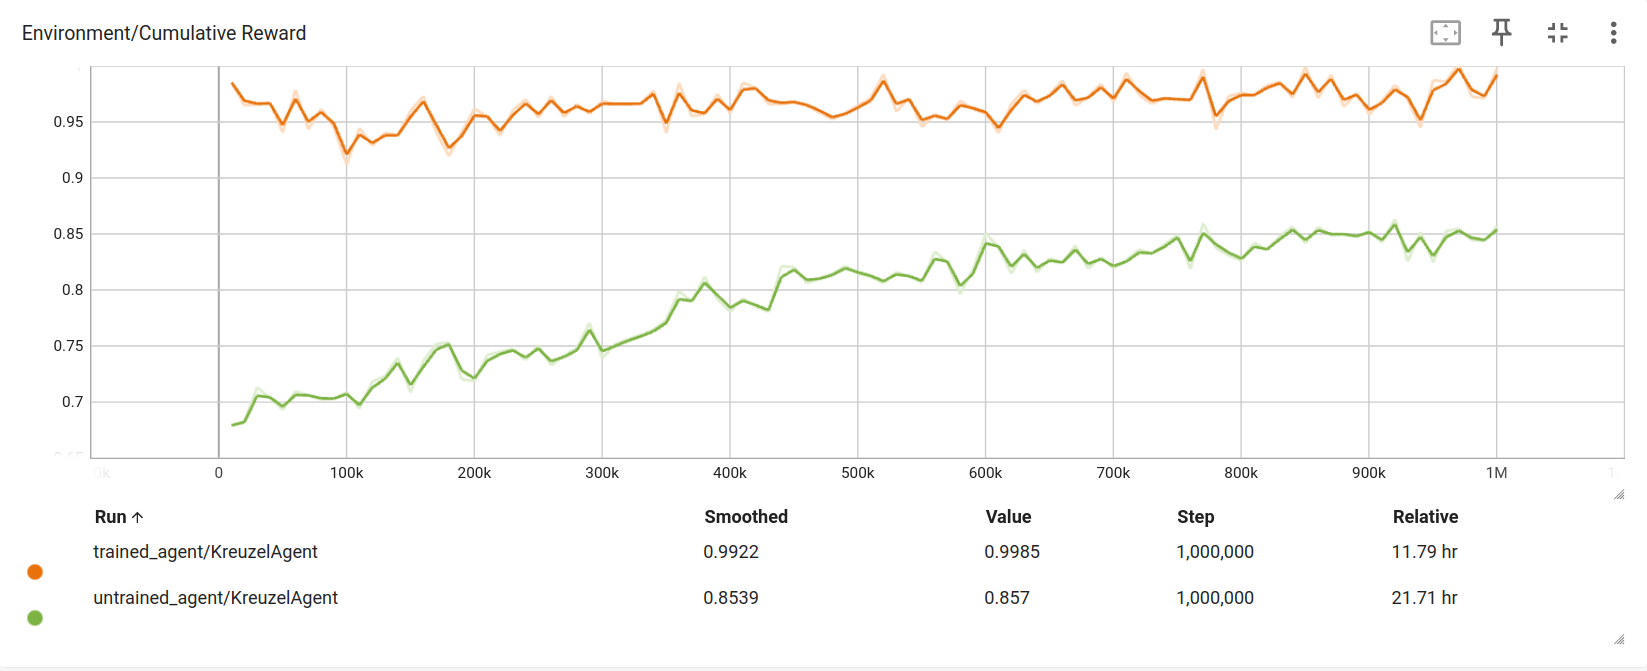
\includegraphics[scale=0.3]{Bilder/vergleich_untrained_vs_trained.png}
    \caption{Übersicht der gesammelten Belohnungen}
\end{figure}


\subsection{Trainiert vs Training mit Sonderfeldern}
In diesem Experiment wurden die erreichten Puntke und Rewards des normal trainierten Agenten gegenüber einem Agenten, welcher mit Sonderfeldern trainiert wurde gegenüber gestellt.
Diese speziellen Felder waren einheitlich in die verschiedenen Farben eingefärbt bzw jedes Feld wurde mit Sternfeldern versehen. Dies sollte dazu führen, dass der Agent besser zuweisen kann welche Stellen im Observationsvektor für welche Information zuständig sind.

Das Training mit speziellen Feldern führte zu einer Verschlechterung des Ergebnisses wie die zwei nachfolgenden Grafiken zeigen.


\begin{figure}[!t]
    \centering
    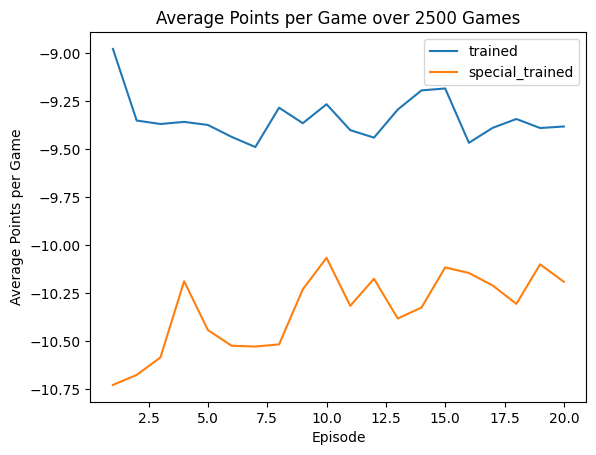
\includegraphics[scale=0.6]{Bilder/special_trained_vs_trained.png}
    \caption{Durchscnbitt der erreichten Punkte beides Agenten}
\end{figure}


\subsection{Trainiert vs Training mit mehr Spielzügen}

In diesem Exderiment sollte der trainierte Agent das mit mehr zur Verfügung stehenden Spielzügen absolvieren. Dies hat zur Folge, dass während des Trainings häufiger zur Puntkewertung kommt und der Agent auf diese Ziele hin arbeiten kann.
Wie die Grafiken zeigen, hatte das Experiment eine Verbesserung der Ergebnisse zur Folge.


\begin{figure}[!t]
    \centering
    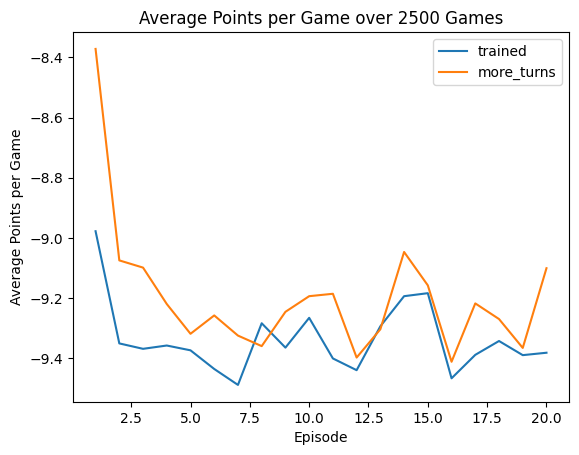
\includegraphics[scale=0.3]{Bilder/moreTurnsVsTrained.png}
    \caption{Durchschnitt der gesammelten Punkte}
\end{figure}


\subsection{Überprüfung auf Overfitting}
In diesem Experiment, sollte der Agent auf Overfitting überprüft werden. trainierte und untrainierter Agent spielten das Spiel nach normalen Spielregeln auf einem anderen Spielfeld.
In den Grafiken ist erkennbar, dass beide Agenten ungefähr die selben Rewards gesammelten haben. Der untraineirte Agent konnte im Durchschnitt jedoch etwas mehr Punkte sammeln.
Dies schließt darauf, dass der Agent tatsächlich nur auf dem im Training verwendeten Spielfeld gut performen kann und neue SPielfelder erst erlernen muss.

Interessant ist weiterhin, dass der Durchschnitt aller Punkte etwa 2 Punkte über dem des anderen SPielfeldes liegt, was auf eine höhere Schwierigkeit des anderen SPielfeldes hinweist.


\begin{figure}[!t]
    \centering
    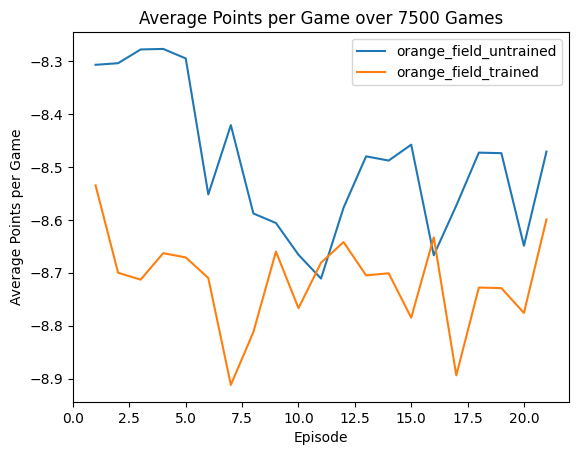
\includegraphics[scale=0.6]{Bilder/orange_field_evaluation.png}
    \caption{durchschnitt an gesammelten Punkten}
\end{figure}
\begin{figure}[!t]
    \centering
    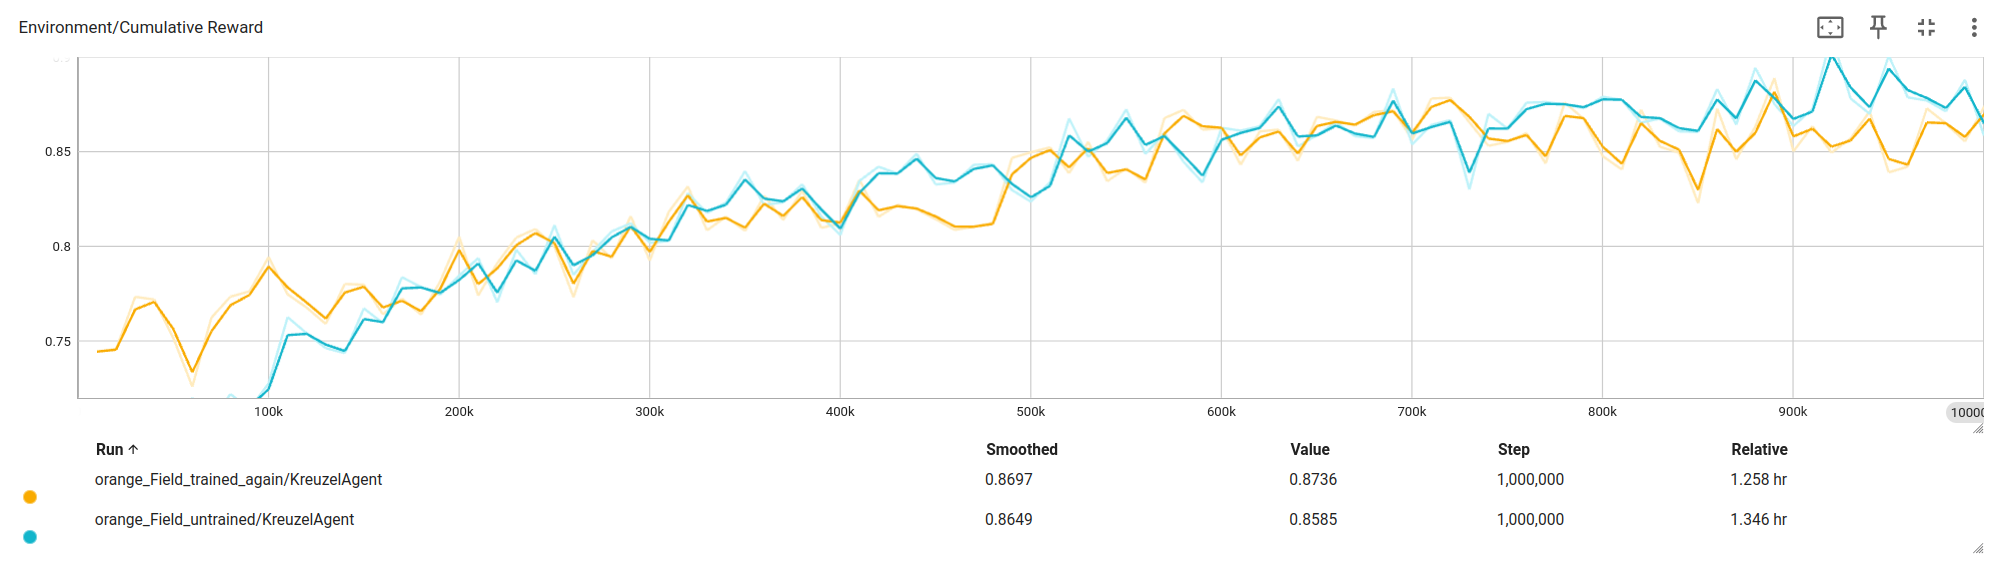
\includegraphics[scale=0.3]{Bilder/orange_field_trained_vs_untrained.png}
    \caption{gesammelte Rewards der beiden Agenten}
\end{figure}

\subsection{Training Auswahl KoordinatenPicker}
Da der Agent keine großen Fortschritte erzielen konnte, entschied ich den Agenten das erste Feld durch Koordinaten zu wählen.
Dies setzte Vorraus, dass die Koordinaten der einzelnen Felder in die Observations mit aufgenommen werdne musste und die Observations noch größer wurden.
Damit der Agent lernen kann, welche Kooordinaten zu welchen Feldern gehören, entschied ic hmic hdazu ihn auf einem Spielfeld trainieren zu lassen, wo alle Teilfelder verfügbar sind.
Rewards wurden vergeben für Valide ausgewählte Felder, in Abhängigkeit der gewürfelten Zahlen.

Im nächsten Schritt wird dieses vortrainierte NN genutzt um das Spiel mit richtigen Regeln zu spielen.
